\subsection{Path following}\label{sec:prob2.2}
\begin{wrapfigure}{r}{0.5 \textwidth}
    \begin{center}
    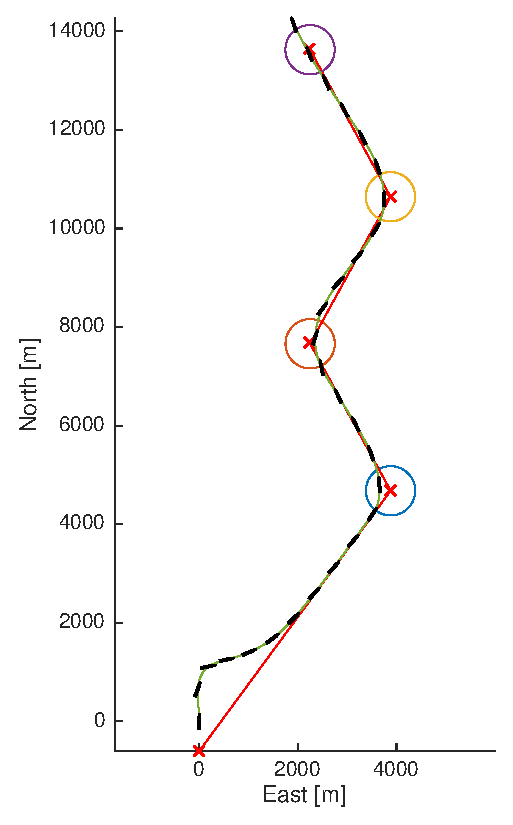
\includegraphics[width=0.7\textwidth]{task2.3/Task2_3-1}
    \caption{Path following}
    \end{center}
    \label{fig:2.3-path}
\end{wrapfigure}

We implemented a lookahead-based steering law, based on figure (10.10) in Fossen (2011). The desired course $\chi_d$ is made up of two parts, a path-angle $\chi_p$ and a cross-track error correction $\chi_r$. The cross-track error correction is essentially a PI-controller, normalized with an inverse tangent. The proportional gain is the inverse of the lookahead distance.
\begin{equation}
	K_p = \frac{1}{\Delta_s}
\end{equation}

The integral effect of the controller is quite complex, since we only want the integrator to compensate for small slow-changing disturbances like wind and current. To achieve this, we made this integral structure:

\begin{equation}
\begin{split}
	\chi_d &= \chi_p + \chi_r \\
	\chi_r &= atan(P - I) \\
	P &= K_p e \\
	I &= \int K_i e_i \\
	e_i &=
\end{split}
\end{equation}


\begin{figure}[b]
    \centering
    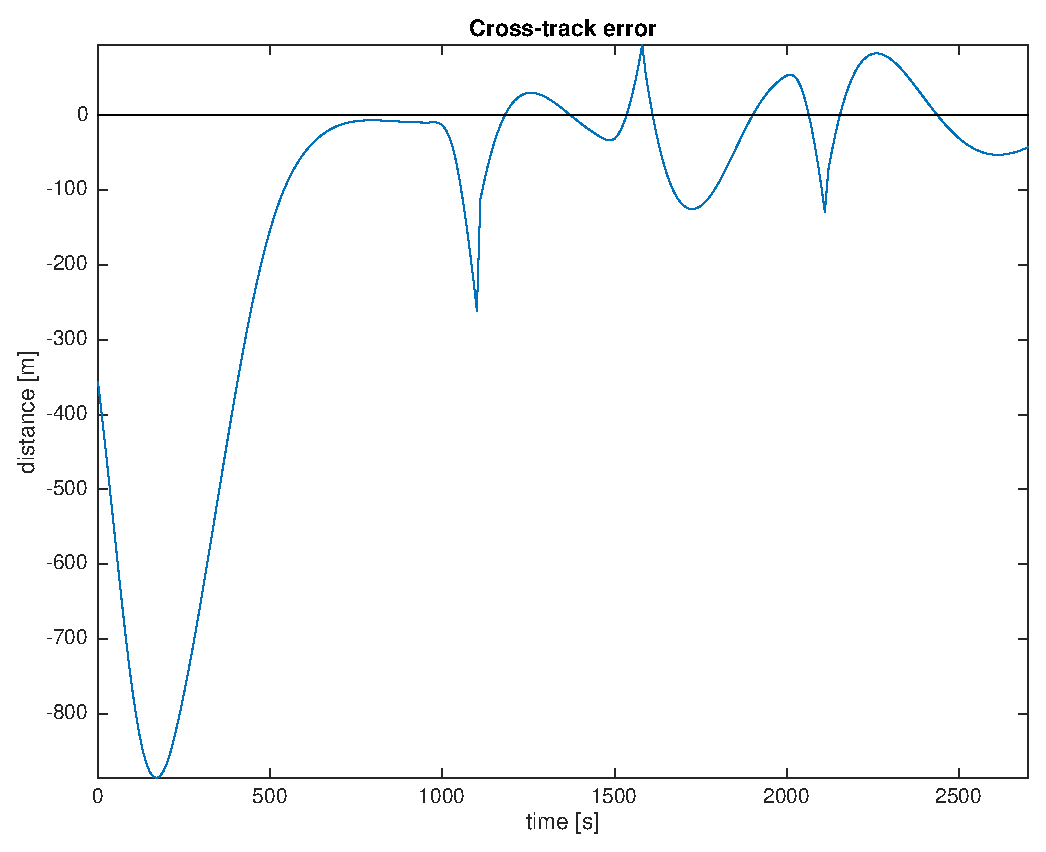
\includegraphics[width=0.8 \textwidth]{task2.3/Task2_3-2}
    \caption{Cross-track error}
    \label{fig:2.3-error}
\end{figure}